%%====================================================================
\section{Software Description}
\label{sec:description}

\subsection{System Architecture}

ResearchShop is a cross-platform desktop application and a command-line utility built with Electron~\cite{electron_docs} (TypeScript/React frontend) and Python 3.11+ (extraction pipeline backend). The desktop process and Python pipeline run on the user's machine with no ResearchShop server infrastructure. The workflow \DIFdelbegin \DIFdel{utilizes }\DIFdelend{} \DIFaddbegin \DIFadd{uses }\DIFaddend{} direct external calls to \DIFdelbegin \DIFdel{NCBI Entrez}\DIFdelend{} \DIFaddbegin \DIFadd{PubMed through NCBI Entrez E-utilities~}\cite{ncbi_eutilities_help}\DIFaddend , PubTator3, PubMed Central, Europe PMC, and Google Gemini as required for paper discovery, open-access retrieval, NER, and LLM extraction. Users provide their own Gemini API key and NCBI Entrez email.

The frontend communicates with the Python pipeline via an IPC (Inter-Process Communication) bridge. The pipeline process emits structured JSON messages on stdout (\texttt{PROGRESS:\{...\}}, \texttt{LOG:\{...\}}, \texttt{RESULT:\{...\}}) which the Electron main process parses and forwards to the React renderer. Secrets (API key, email) are passed as environment variables to the spawned Python process, never as command-line arguments.

The pipeline follows the seven implementation domains shown in Figure~\ref{fig:architecture}.

\LucasNote{tę listę można by jakoś wprowadzić, bo na razie pojawia się bez wcześniejszej zapowiedzi w tekście, poza wzmianką w przedostatnim akapicie}
\LucasNote{czy dobrze rozwinąłem, co to jest Entrez?}
\LucasNote{może "full capped result set before pagination" jest zbędne?}
\LucasNote{czy to jest stała konfiguracyjna w naszym oprogramowaniu? czy można zmienić tę wartość?}
\DIFdelbegin
\begin{enumerate}[leftmargin=*,itemsep=2pt]
    \item \DIFdel{\textbf{Paper selection.} PubMed records are retrieved through NCBI Entrez E-utilities and ranked using title/abstract relevance, citation information, and journal quartiles. All records remain visible, and user-supplied PMID lists are not widened.}
    \item \DIFdel{\textbf{Open-access filtering.} Query mode considers a configurable pool of open-access candidates before selecting the requested top-$N$; selected PMIDs proceed only when full text is available.}
    \item \DIFdel{\textbf{Paper reading.} PMC JATS XML is preferred, with Europe PMC XML as fallback; sections, tables, captions, image links, and supplementary metadata are retained where available.}
    \item \DIFdel{\textbf{Candidate discovery.} PubTator3 NER, deterministic HGNC symbol/alias scanning, and a full-text LLM pass propose candidates. Optional recall and figure passes can extend the set.}
    \item \DIFdel{\textbf{Detail extraction.} Gemini fills the custom schema and supplies source citations. PubTator and HGNC candidates are included as seeds. The default model is \texttt{gemini-2.5-flash-lite}, and model identifiers are configurable.}
    \item \DIFdel{\textbf{Validation.} A bundled HGNC database, HGNC REST, and MyGene.info support normalization; source grounding, citation checks, HGVS matching, and confidence gates determine exportability.}
    \item \DIFdel{\textbf{Output writing.} A bounded worker pool applies a configurable per-paper timeout and writes deduplicated CSV, JSON, XLSX, metadata, trace, and candidate-audit artifacts.}
\end{enumerate}
\DIFdelend

\DIFaddbegin
\begin{enumerate}[leftmargin=*,itemsep=1pt]
    \item \DIFadd{\textbf{Paper selection} retrieves PubMed records through NCBI Entrez E-utilities~\cite{ncbi_eutilities_help}. Topic results are ranked by gene relevance and capped impact signals; user-supplied PMID lists are unchanged.}
    \item \DIFadd{\textbf{Open-access filtering} admits only papers whose full text can be fetched from PMC or Europe PMC.}
    \item \DIFadd{\textbf{Paper reading} preserves JATS sections, tables, captions, image links, and supplementary metadata where available.}
    \item \DIFadd{\textbf{Candidate discovery} combines PubTator3 NER~\cite{wei2024pubtator3}, deterministic HGNC scanning, and a full-text LLM pass.}
    \item \DIFadd{\textbf{Detail extraction} fills the user-defined schema and requests source quotations. The default model is \texttt{gemini-2.5-flash-lite}; model identifiers are configurable~\cite{google_gemini_models}.}
    \item \DIFadd{\textbf{Validation} applies a versioned bundled HGNC snapshot~\cite{braschi2019genenames}, HGNC REST~\cite{hgnc_rest_docs}, MyGene.info~\cite{wu2013biogps}, source grounding, citation checks, and HGVS matching.}
    \item \DIFadd{\textbf{Output writing} uses a bounded worker pool and configurable timeout, then writes primary tables and audit artifacts.}
\end{enumerate}
\DIFaddend

\begin{figure*}[t]
    \centering
    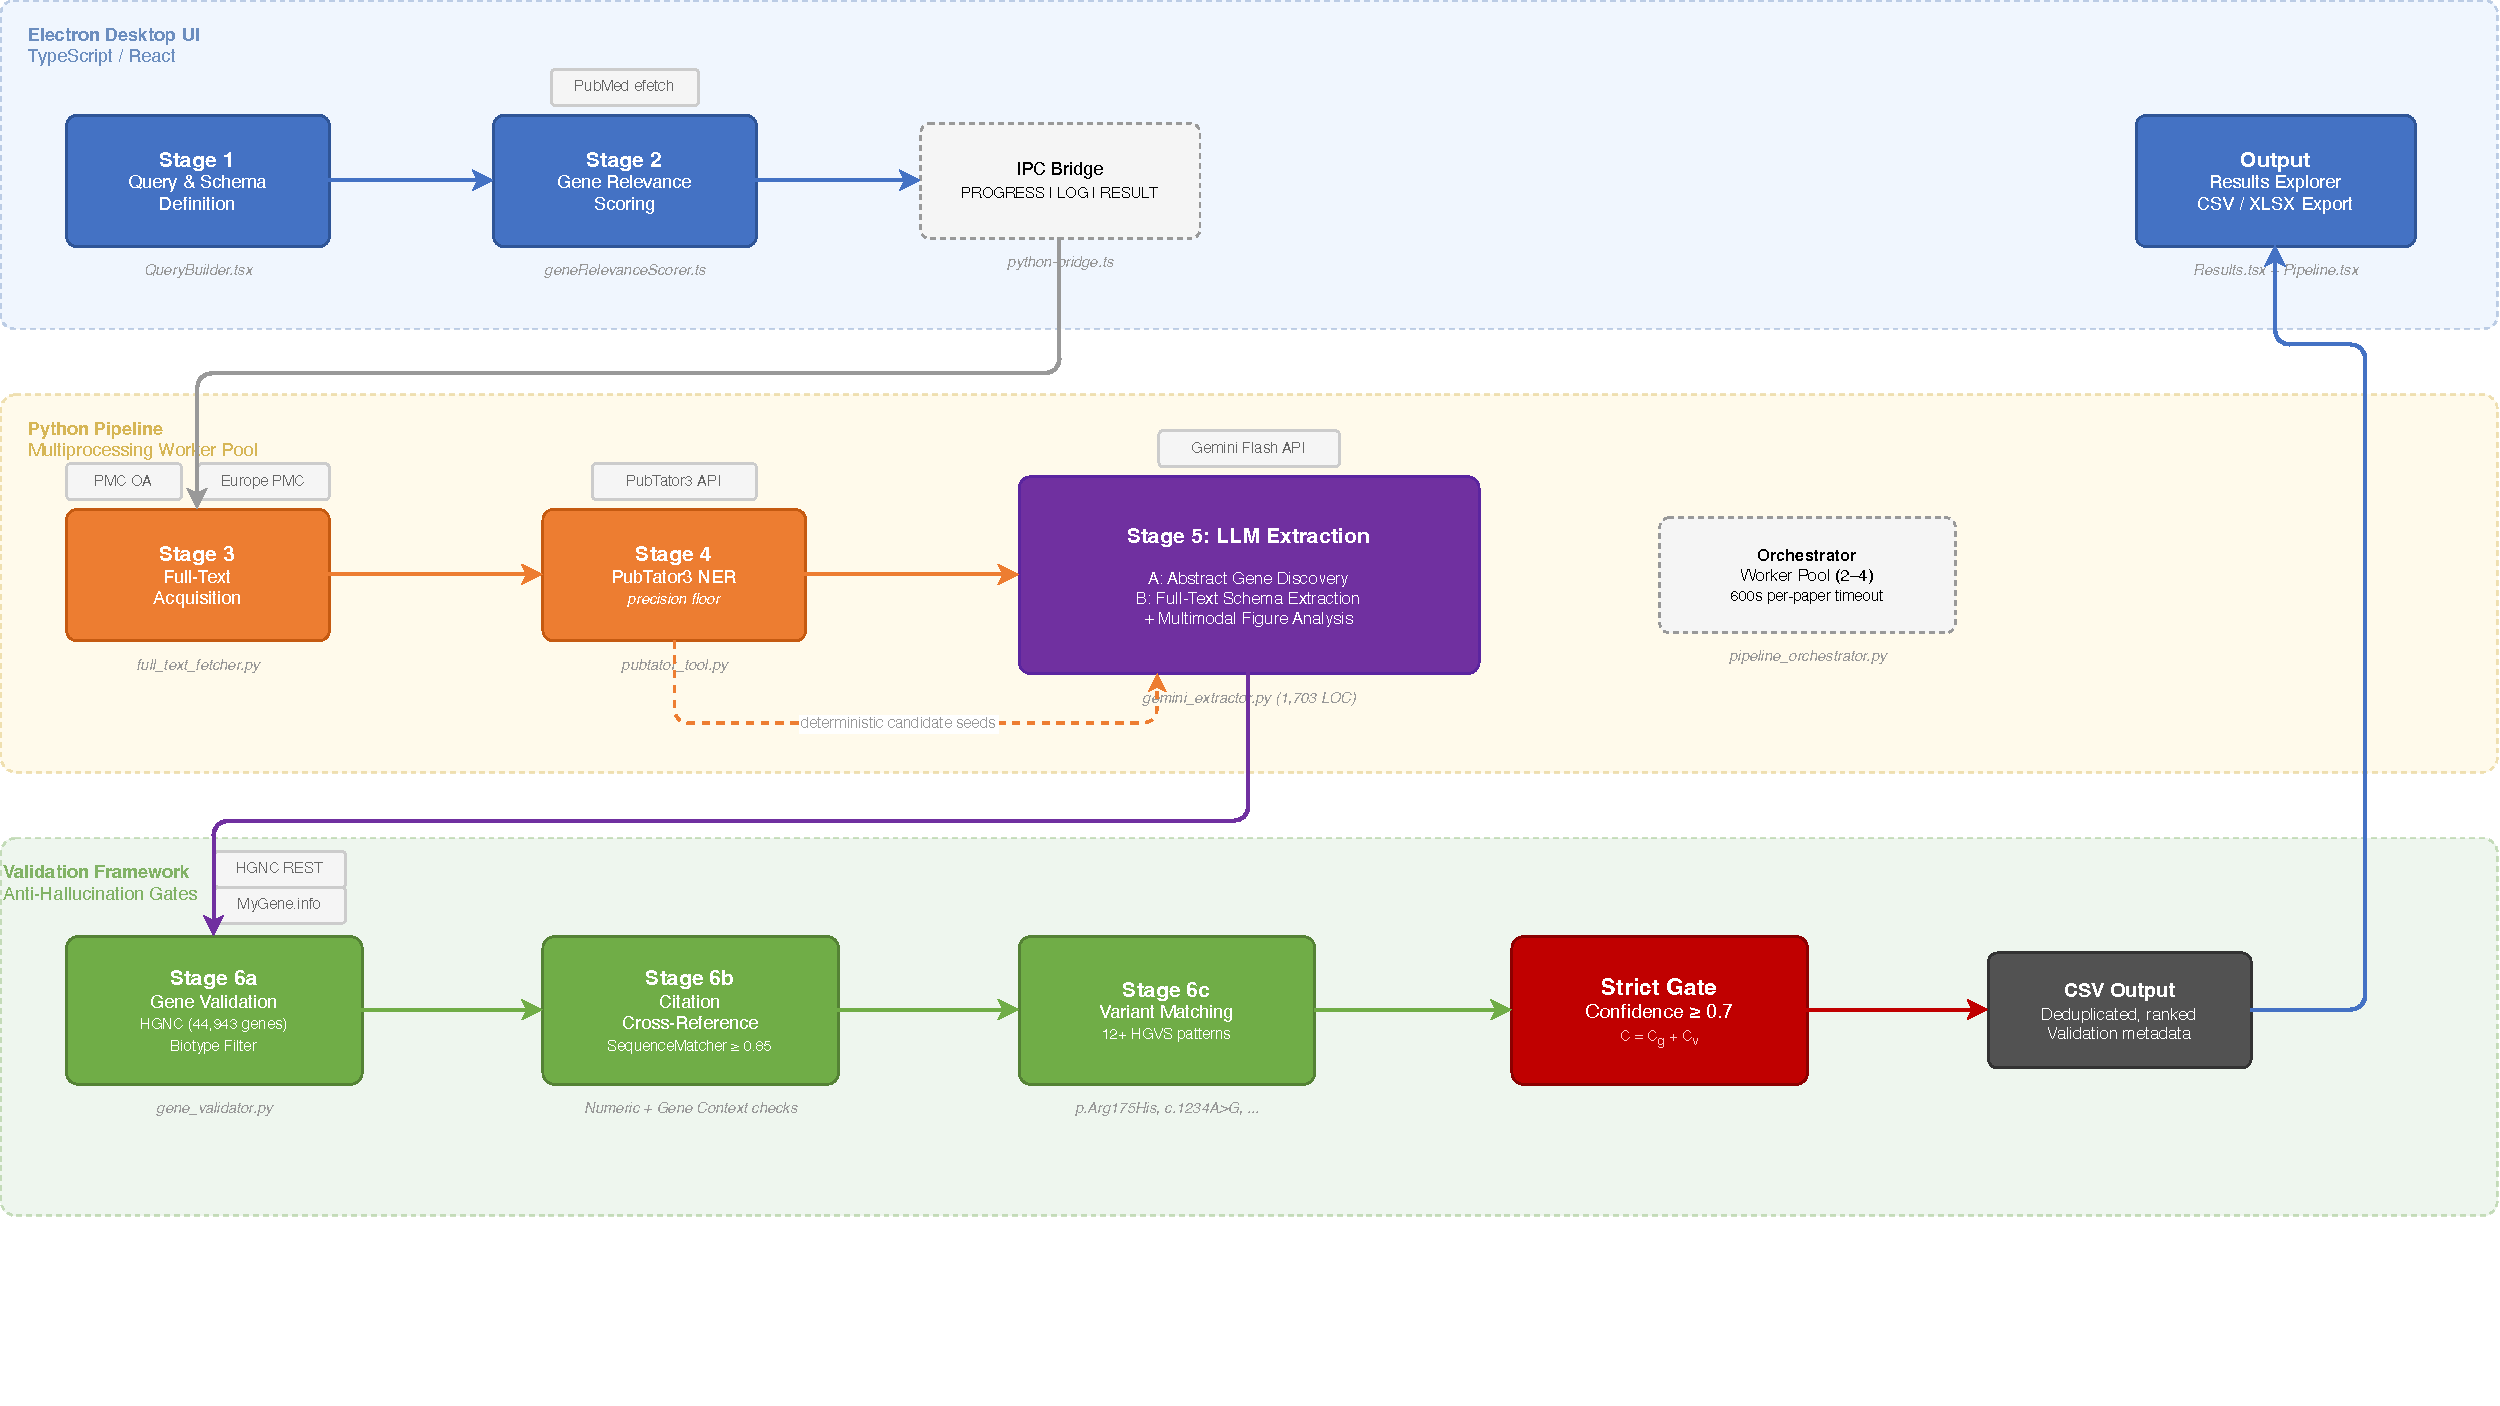
\includegraphics[width=0.94\textwidth]{figures/pipeline_tikz.pdf}
    \caption{ResearchShop system architecture. The Electron UI layer (top) handles query input, gene relevance scoring, and results display. The Python pipeline (middle) executes open-access full-text reading, candidate discovery, LLM-based detail extraction, and output writing. The validation framework (bottom) applies gene symbol verification, source grounding, citation cross-referencing, variant checking, and a strict confidence gate ($\geq$0.7) before output.}
    \label{fig:architecture}
\end{figure*}

Figure~\ref{fig:architecture} separates proposal, extraction, and validation because these stages have different error profiles. The UI and paper-selection stages decide \emph{which papers} to process; the candidate-discovery stages decide \emph{which gene labels} deserve attention; the LLM stage fills user-defined fields only after receiving source-derived candidates; and the validation layer decides \emph{which rows} are safe enough for the primary export. Hallucinations are constrained at three points: the LLM is seeded with candidates that already came from the source text, every returned gene must be grounded back to the article, and citation-bearing fields must point to recoverable source passages before export.

\subsection{Hybrid NER-LLM Architecture}

\DIFdelbegin
\DIFdel{NER identifies biomedical entities but generally does not answer the user-facing question: what did the paper claim about the gene? Pure LLM extraction can fill richer schemas, but it may attach a plausible claim to the wrong gene or to no source passage. ResearchShop therefore assigns PubTator3, HGNC scanning, the LLM, and validation separate roles. PubTator3 supplies a precision-oriented entity set; HGNC scanning adds source-grounded recall; the LLM supplies contextual fields and quotations; and deterministic checks record why each row passed or failed. Source-derived candidates are injected into the prompt, and every returned gene is searched in the article using its canonical symbol, aliases, biomedical mention bridges, and raw model label.}
\DIFdelend

\DIFaddbegin
\DIFadd{The hybrid design separates entity detection from contextual extraction. PubTator3 supplies normalized biomedical entities, while deterministic HGNC scanning recovers symbols and aliases missed by NER. The LLM fills researcher-defined fields for these source-derived candidates, but its rows remain untrusted until identifier, text, citation, and variant checks pass. Pure NER therefore lacks the requested context; pure LLM extraction lacks deterministic evidence constraints.}
\DIFaddend

\subsection{Schema-Driven Extraction}

Users define custom output columns as natural-language descriptions. For example, researchers might specify:

\begin{itemize}[itemsep=1pt]
    \item \textbf{Key Finding}: Main research finding for this gene
    \item \textbf{Statistical Evidence}: p-values, odds ratios, confidence intervals
    \item \textbf{Functional Impact}: Effect on protein function or pathway
\end{itemize}

The pipeline dynamically constructs LLM prompts incorporating these column definitions, enabling researchers to customise extraction for different contexts (pharmacogenomics, rare diseases, cancer genomics) without code modifications. Schema-driven extraction was chosen instead of free-form summarisation because it makes the output contract explicit: every run has named fields, predictable column order, companion citation columns, and validation metadata that can be checked programmatically. For each extracted value, the LLM is required to provide a verbatim citation from the source text. If a requested field is not supported by the paper, the expected behaviour is an empty field rather than a speculative answer.

\subsection{Desktop Application}
\label{subsec:desktop}

The application is packaged with electron-builder. The current public release provides a macOS \texttt{.dmg}; Windows \texttt{.exe} and Linux \texttt{.AppImage}/\texttt{.deb} targets are supported by the build configuration and remain part of release validation. On first launch, the application automatically creates a Python virtual environment and installs pipeline dependencies.

The GUI provides:
\begin{itemize}[itemsep=1pt]
    \item \textbf{Onboarding wizard:} API key validation, output directory selection, research-use disclaimer.
    \item \textbf{Query builder:} PubMed search with relevance scoring and paper selection.
    \item \textbf{Live pipeline monitor:} Real-time progress, per-stage breakdown, Gemini API usage tracking, and technical logs for debugging failed runs.
    \item \textbf{Results explorer:} Sortable table with confidence badges (CORROBORATED, SUPPORTED, LIMITED EVIDENCE, NEEDS REVIEW), plain-language confidence explanations, evidence/provenance fields, and CSV/XLSX export.
\end{itemize}

\begin{table}[t]
\centering
\footnotesize
\setlength{\tabcolsep}{3pt}
\renewcommand{\arraystretch}{1.05}
\begin{tabularx}{\columnwidth}{>{\raggedright\arraybackslash}p{2.35cm} X}
\toprule
\textbf{Badge} & \textbf{Meaning} \\
\midrule
\textsc{CORROBORATED} & Multiple checks agree and matched supporting text was found. \\
\textsc{SUPPORTED} & Valid gene appears in the paper; some evidence may need inspection. \\
\textsc{LIMITED EVIDENCE} & Support is weak, incomplete, or available only in limited context. \\
\textsc{NEEDS REVIEW} & Important check failed, extraction was incomplete, or manual review is required. \\
\bottomrule
\end{tabularx}
\caption{Confidence badges are review cues, not clinical assertions.}
\label{tab:confidence_badges}
\end{table}

Security measures include OS-keychain-backed API key encryption (via Electron \texttt{safeStorage}), Content Security Policy headers, IPC path traversal validation, sandboxed renderer, and PMID input sanitisation.

\FloatBarrier
\subsection{Validation Framework}
\label{subsec:validation}

\DIFdelbegin
\DIFdel{The validation framework treats the LLM output as an untrusted draft. The model may propose structured rows and fill user-defined fields, but the pipeline decides whether a row is exportable by re-checking it against source text, controlled vocabularies, and deterministic pattern matchers. A second LLM could provide another fluent judgement, but it would not solve the core auditability problem.}
\DIFdelend

\subsubsection{LLM Output Validation Heuristics}

\DIFdelbegin
\DIFdel{For each paper, validation begins with a constrained candidate set assembled from PubTator3 entities, deterministic HGNC symbol and alias scanning, and LLM candidate discovery. Candidate generation asks which genes might be relevant; detail extraction asks what the paper says about those genes; validation asks whether each row is grounded enough to export. The returned rows are processed by the following deterministic heuristics:}
\begin{enumerate}[itemsep=2pt]
    \item \DIFdel{\textbf{Identifier normalisation.} Map the reported string to an HGNC-approved symbol and retain aliases as provenance.}
    \item \DIFdel{\textbf{Source presence.} Require the canonical symbol, an alias, or the raw LLM mention in the fetched text.}
    \item \DIFdel{\textbf{Citation anchoring.} Match each evidence quotation back to the article.}
    \item \DIFdel{\textbf{Local gene context.} Require the relevant gene near the matched quotation.}
    \item \DIFdel{\textbf{Numerical preservation.} Require numeric tokens in a quotation to occur in the source passage.}
    \item \DIFdel{\textbf{Variant sanity check.} Test variant-like strings against HGVS-oriented patterns.}
    \item \DIFdel{\textbf{Hard gates before export.} Exclude rows that fail identifier, source, or citation requirements.}
    \item \DIFdel{\textbf{Confidence label and audit trail.} Score rows that pass the hard gates and record every exclusion.}
\end{enumerate}
\DIFdel{These heuristics bound the LLM's role rather than replacing expert curation: the model may summarize and structure evidence, but exported rows must remain tied to identifiers and source passages that ResearchShop can locate in the paper.}
\DIFdelend
\LucasNote{Może informację o tym, że jest to CSV można tu pominąć?}

\DIFaddbegin
\DIFadd{Candidate generation, schema filling, and validation are separate operations. PubTator3, HGNC scanning, and LLM discovery propose genes; the detail call supplies field values and quotations; the deterministic rules in Table~\ref{tab:llm_validation_decisions} decide whether a row is exportable. This division limits two complementary errors: pure LLM extraction can add plausible but unsupported rows, whereas rigid entity filtering can discard genuine findings expressed through aliases or unusual context. ResearchShop therefore retains rejected candidates in audit files while admitting only source-grounded rows to the primary export.}
\DIFaddend

\begin{table*}[t]
\centering
\small
\setlength{\tabcolsep}{5pt}
\renewcommand{\arraystretch}{1.08}
\begin{tabularx}{\textwidth}{>{\raggedright\arraybackslash}p{2.7cm} >{\raggedright\arraybackslash}X >{\raggedright\arraybackslash}p{3.5cm} >{\raggedright\arraybackslash}p{3.0cm}}
\toprule
\textbf{Check} & \textbf{Decision rule} & \textbf{Failure addressed} & \textbf{Primary output action} \\
\midrule
HGNC normalization & Map the reported gene string to an approved symbol using the local HGNC snapshot, aliases, previous symbols, HGNC REST, or MyGene.info fallback. Fuzzy matches may suggest corrections but are not authoritative evidence. & Invalid symbols, obsolete labels, ambiguous aliases, and typographic near-misses. & Required gate; unresolved symbols are excluded from the primary \DIFdelbeginFL \DIFdelFL{CSV}\DIFdelendFL{} \DIFaddbeginFL \DIFaddFL{export}\DIFaddendFL . \\
Source grounding & Require the canonical symbol, an alias, or the raw LLM mention to occur in fetched article text. & Real but off-paper genes introduced from model prior knowledge. & Required gate; failures go to review/drop artifacts. \\
Citation anchoring & Match the LLM evidence quote to article text after normalization using exact matching or dense \texttt{SequenceMatcher} matching~\cite{python_difflib,ratcliff1988gestalt}. & Fabricated, paraphrased, or unlocatable citations. & Required row-level gate when citation fields are present; at least one supplied citation must ground. \\
Local gene context & Require the gene symbol or accepted alias within the citation context window. & Correct source sentence attached to the wrong gene in a multi-gene paper. & Enforced inside citation validation. \\
Numeric preservation & Require source matches for p-values, odds ratios, percentages, cohort sizes, positions, and other numeric tokens. & Altered statistics, rounded values, or invented quantitative detail. & Enforced inside citation validation when numeric claims are present. \\
Variant validation & Match variant-like strings against HGVS-oriented protein, coding, genomic, splice, indel, copy-number, translocation, and cytogenetic patterns. & Malformed variants or unsupported nomenclature. & Variant confidence only; unvalidated variants remain review metadata. \\
Confidence gate & After required gates pass, export rows only when $C_{\mathrm{total}} \geq 0.7$. & Weakly supported associations after identifier and evidence checks. & Below-threshold rows are omitted and audited. \\
\bottomrule
\end{tabularx}
\caption{Deterministic decision model used to validate LLM-generated extraction rows before export.}
\label{tab:llm_validation_decisions}
\end{table*}

\DIFdelbegin
\DIFdel{The thresholds in Table~\ref{tab:llm_validation_decisions} are engineering heuristics selected to favour precision in the default export, not claims about biological truth. The 0.85 citation threshold permits XML, Unicode, and line-wrapping drift while rejecting paraphrases. The $\pm$1,500-character context window covers captions, table lead-ins, and adjacent paragraphs without accepting article-level co-mentions as evidence. The 0.7 confidence threshold is a conservative export cutoff applied only after required hard gates pass, not a calibrated probability.}
\DIFdelend
\LucasNote{Co należy rozumieć przez biologicla constants?}

\DIFdelbegin
\DIFdel{\textbf{Gene symbol validation.} Every extracted gene is checked against a bundled HGNC snapshot, HGNC REST, and MyGene.info. Fuzzy matching suggests corrections but is not authoritative. Biotype is retained as metadata, and valid non-protein-coding symbols are not rejected.}

\DIFdel{\textbf{Grounding and citation checks.} The canonical symbol, aliases, and raw model label are searched in the paper. Citations are checked by exact or dense sequence matching; short quotations require exact matches. Numeric consistency, local gene context, and symmetric encoding normalization are also enforced.}

\DIFdel{\textbf{Variant and confidence checks.} Variant strings are compared with HGVS-oriented patterns. Rows must first pass HGNC normalization, source grounding, and citation anchoring. A confidence score is then computed from gene and variant validation, and rows below 0.7 are excluded from the primary export.}
\DIFdelend

\DIFaddbegin
\DIFadd{Identifier validation queries the bundled HGNC snapshot first, followed by HGNC REST and MyGene.info; fuzzy matches are suggestions only~\cite{braschi2019genenames,hgnc_rest_docs,wu2013biogps,python_difflib}. The source-grounding check then requires the canonical symbol, an accepted alias, or the raw model label in the fetched article. This blocks real genes recalled from model training but absent from the paper.}

\DIFadd{Evidence quotations are matched exactly or with normalized \texttt{SequenceMatcher} similarity of at least 0.85~\cite{python_difflib,ratcliff1988gestalt}. Quotations shorter than five words require exact matches. Numeric tokens must be preserved, and the relevant gene must occur within a $\pm$1,500-character source window. These are conservative engineering settings, not biologically calibrated thresholds: 0.85 tolerates extraction-format drift, while the bounded window covers adjacent paragraphs and table or caption lead-ins without accepting article-wide co-mentions.}

\DIFadd{Variant strings are compared with HGVS-oriented patterns~\cite{denDunnen2016hgvs}. Rows must pass identifier, source, and applicable citation gates before scoring. For rows that pass,}
\DIFaddend
\begin{equation}
C_{\mathrm{total}} = C_g + C_v
\label{eq:confidence}
\end{equation}
\DIFaddbegin
\DIFadd{where $C_g=0.7$ for a validated gene ($1.0$ for gene-only rows) and $C_v=0.3$ for a syntactically valid variant. The 0.7 export cutoff is therefore a workflow heuristic, not a probability of biological correctness. Failed rows remain in audit artifacts for review.}
\DIFaddend
